% SC4051 --- Chapter 2: Time, Clocks and Consistency (0->100)
\chapter{Time, Clocks and Consistency}
\label{ch:time}

\begin{quote}
\emph{``Time is what we read from a clock.''} --- Einstein, operationally. In a distributed system there is no single clock to read, so we must invent notions of ``before'' that we can actually measure.
\end{quote}

\noindent\fbox{\parbox{\dimexpr\linewidth-2\fboxsep-2\fboxrule}{%
\textbf{From zero: clocks and causality from scratch.} We start with why wall clocks fail (drift, NTP limits), define the happens-before relation, then build logical and vector clocks that capture causality without physical time. We close by mapping the zoo of consistency models onto what applications actually need.}}
\vspace{0.4em}

\section*{Learning Outcomes}
After this chapter you will be able to:
\begin{enumerate}[label=(L\arabic*)]
    \item explain clock drift, skew and NTP/PTP bounds (TrueTime);
    \item define Lamport's happens-before and derive logical clock rules;
    \item maintain and compare vector clocks to detect causality vs.\ concurrency;
    \item order consistency models from strong to weak (linearizable $\to$ eventual);
    \item choose a consistency level for a given application invariant.
\end{enumerate}

% ============================================================
\section{Physical Time Is Unreliable}
\label{sec:physical}
Two quartz oscillators drift apart by $10$--$100$ parts per million; after a day that is seconds of skew. NTP synchronises to tens of milliseconds over the WAN (sub-millisecond on LAN); PTP with hardware timestamps reaches microseconds; Google's TrueTime (Spanner) exposes an \emph{interval} $[earliest, latest]$ rather than a point, with typical uncertainty $\epsilon\approx 2$--$7$\,ms. No protocol can make clocks agree exactly in the presence of uncertain delay---it can only bound the error.

That bound matters. If node $A$ timestamps an event at $t_A$ and $B$ at $t_B$, $t_A < t_B$ does \emph{not} mean $A$ happened first when $|t_A-t_B|<\epsilon$. Systems that order by wall-clock alone (e.g., ``last writer wins'' with client clocks) silently lose updates when clocks skew.

\begin{figure}[h]
\centering
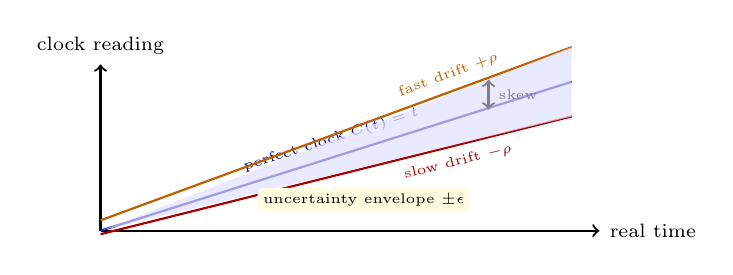
\begin{tikzpicture}[scale=0.88, every node/.style={font=\scriptsize},
  ax/.style={->,thick}]
\draw[ax] (0,0) -- (7.2,0) node[right] {real time};
\draw[ax] (0,0) -- (0,2.4) node[above] {clock reading};
\draw[thick,blue!60!black] (0,0) -- (6.8,2.15) node[midway,above,sloped,font=\tiny] {perfect clock $C(t)=t$};
\draw[thick,orange!75!black] (0,0.15) -- (6.8,2.65) node[near end,above,sloped,font=\tiny] {fast drift $+\rho$};
\draw[thick,red!65!black] (0,-0.05) -- (6.8,1.65) node[near end,below,sloped,font=\tiny] {slow drift $-\rho$};
\fill[blue!12,opacity=0.7] (0,0) -- (6.8,2.65) -- (6.8,1.65) -- cycle;
\node[font=\tiny,fill=yellow!12,rounded corners=2pt,inner sep=2pt] at (3.8,0.45) {uncertainty envelope $\pm\epsilon$};
\draw[<->,thick,gray] (5.6,1.75) -- (5.6,2.18) node[midway,right,font=\tiny] {skew};
\end{tikzpicture}
\caption{Physical clocks diverge within a drift envelope. NTP/PTP/TrueTime bound the skew but never eliminate it.}
\label{fig:drift}
\end{figure}

TrueTime's insight: instead of pretending $now$ is a point, return $[now-\epsilon, now+\epsilon]$ and make callers wait out the uncertainty before committing. Spanner's commit-wait (Ch.~7) is exactly that: delay commit until $TT.now().latest$ passes the chosen timestamp, so timestamp order respects real-time order.

% ============================================================
\section{Lamport Clocks: Capturing Happens-Before}
\label{sec:lamport}
Lamport (1978) asked what ``before'' can mean without physical time. Define the \emph{happens-before} relation $\to$ as the smallest transitive relation such that (i) if $a$ and $b$ are events on the same process and $a$ precedes $b$, then $a\to b$, and (ii) if $a$ is the send of a message and $b$ is its receive, then $a\to b$. Two events are \emph{concurrent} ($a\parallel b$) if neither $a\to b$ nor $b\to a$.

A \emph{Lamport logical clock} $C$ is a counter per process:
\begin{equation}
\begin{aligned}
\text{local event / send:}&\quad C := C+1 \\
\text{receive of }m\text{ with }C_m:&\quad C := \max(C, C_m)+1;\ \text{deliver }m
\end{aligned}
\end{equation}
with $C_m$ piggybacked on $m$.

\begin{theorem}[Clock condition]
If $a\to b$ then $C(a) < C(b)$. The converse does not hold.
\end{theorem}
So equal or smaller clocks do not prove causality---they only rule it out in one direction. That gap motivates vector clocks.

\begin{figure}[h]
\centering
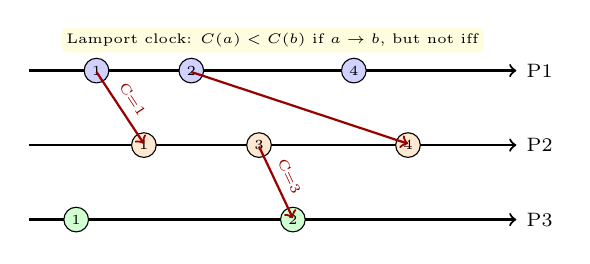
\begin{tikzpicture}[scale=0.86, every node/.style={font=\scriptsize},
  proc/.style={thick,->}]
\draw[proc] (0,2.2) -- (7.2,2.2) node[right] {P1};
\draw[proc] (0,1.1) -- (7.2,1.1) node[right] {P2};
\draw[proc] (0,0) -- (7.2,0) node[right] {P3};
% events
\foreach \x/\l in {1.0/1,2.4/2,4.8/4} \node[draw,circle,fill=blue!18,inner sep=1.5pt] at (\x,2.2) {\tiny\l};
\foreach \x/\l in {1.7/1,3.4/3,5.6/4} \node[draw,circle,fill=orange!18,inner sep=1.5pt] at (\x,1.1) {\tiny\l};
\foreach \x/\l in {0.7/1,3.9/2} \node[draw,circle,fill=green!18,inner sep=1.5pt] at (\x,0) {\tiny\l};
% messages labeled with Lamport timestamps
\draw[->,thick,red!60!black] (1.0,2.18) -- (1.7,1.12) node[midway,above,sloped,font=\tiny] {C=1};
\draw[->,thick,red!60!black] (3.4,1.08) -- (3.9,0.02) node[midway,above,sloped,font=\tiny] {C=3};
\draw[->,thick,red!60!black] (2.4,2.18) -- (5.6,1.12);
\node[font=\tiny,fill=yellow!12,rounded corners=2pt,inner sep=2pt] at (3.6,2.65) {Lamport clock: $C(a)<C(b)$ if $a\to b$, but not iff};
\end{tikzpicture}
\caption{Lamport clocks along three processes. Messages carry the sender's clock; receivers advance past it. Only the clock condition (one direction) holds.}
\label{fig:lamport}
\end{figure}

Total order from Lamport clocks is obtained by breaking ties with process IDs: $(C(a), pid(a)) < (C(b), pid(b))$. That order respects $\to$ and is useful for mutual exclusion (Lamport's bakery), but it \emph{imposes} order on concurrent events arbitrarily---sometimes you need to know they were concurrent.

% ============================================================
\section{Vector Clocks: Detecting Causality}
\label{sec:vector}
A \emph{vector clock} $VC$ is an array of $n$ counters, one per process. On process $i$:
\begin{equation}
\begin{aligned}
\text{local/send:}&\quad VC[i] := VC[i]+1 \\
\text{receive of }m\text{ with }VC_m:&\quad VC[j]:=\max(VC[j],VC_m[j])\ \forall j;\ VC[i]{+}{+}
\end{aligned}
\end{equation}

Comparison is componentwise:
\begin{equation}
VC(a) < VC(b) \iff \forall k\; VC(a)[k]\le VC(b)[k]\ \land\ \exists k\; VC(a)[k]<VC(b)[k].
\end{equation}

\begin{theorem}[Vector clock characterisation]
$VC(a) < VC(b) \iff a \to b$. \quad $VC(a)\parallel VC(b)$ (incomparable) $\iff a\parallel b$.
\end{theorem}
Thus vector clocks \emph{exactly} capture causality, at cost $O(n)$ per message. Practical systems use optimisations: dotted version vectors, version vectors per key, or causal histories pruned by stability.

\begin{lstlisting}[language=Python]
# Vector clocks: exact causality tracking
class VectorClock:
    def __init__(self, n, pid):
        self.n, self.pid = n, pid
        self.v = [0]*n
    def tick(self):
        self.v[self.pid] += 1
        return list(self.v)
    def send(self):
        self.v[self.pid] += 1
        return list(self.v)          # piggyback on message
    def receive(self, other):
        for i in range(self.n):
            self.v[i] = max(self.v[i], other[i])
        self.v[self.pid] += 1

# Example: 3 processes, concurrent updates detected
a = VectorClock(3, 0); b = VectorClock(3, 1)
a.tick()            # a: [1,0,0]
b.tick()            # b: [0,1,0]  -- incomparable => concurrent
print(a.v, b.v, "concurrent:", not (a.v < b.v or b.v < a.v))

# After b receives from a, b dominates a => causal
msg = a.send()      # a: [2,0,0]
b.receive(msg)      # b: [2,2,0]
print("after receive b=", b.v, " a->b ?", all(x<=y for x,y in zip([2,0,0], b.v)))
\end{lstlisting}

\begin{figure}[h]
\centering
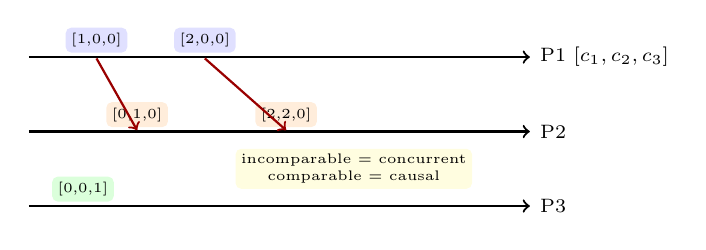
\begin{tikzpicture}[scale=0.86, every node/.style={font=\scriptsize}]
\draw[->,thick] (0,2.2) -- (7.4,2.2) node[right] {P1 $[c_1,c_2,c_3]$};
\draw[->,thick] (0,1.1) -- (7.4,1.1) node[right] {P2};
\draw[->,thick] (0,0) -- (7.4,0) node[right] {P3};
\node[font=\tiny,fill=blue!12,rounded corners=2pt,inner sep=2pt] at (1.0,2.45) {[1,0,0]};
\node[font=\tiny,fill=blue!12,rounded corners=2pt,inner sep=2pt] at (2.6,2.45) {[2,0,0]};
\node[font=\tiny,fill=orange!14,rounded corners=2pt,inner sep=2pt] at (1.6,1.35) {[0,1,0]};
\node[font=\tiny,fill=orange!14,rounded corners=2pt,inner sep=2pt] at (3.8,1.35) {[2,2,0]};
\node[font=\tiny,fill=green!14,rounded corners=2pt,inner sep=2pt] at (0.8,0.25) {[0,0,1]};
\draw[->,thick,red!60!black] (1.0,2.18) -- (1.6,1.12);
\draw[->,thick,red!60!black] (2.6,2.18) -- (3.8,1.12);
\node[font=\tiny,align=center,fill=yellow!12,rounded corners=2pt,inner sep=2pt] at (4.8,0.55) {incomparable = concurrent\\comparable = causal};
\end{tikzpicture}
\caption{Vector clocks on three processes. $[1,0,0]\parallel[0,1,0]$ (concurrent) but $[1,0,0]<[2,2,0]$ (causal).}
\label{fig:vector}
\end{figure}

% ============================================================
\section{Consistency Models}
\label{sec:consistency}
Consistency defines what values a read may return given concurrent writes. Stronger models are easier to program but cost latency and availability.

\begin{description}[leftmargin=1.2em,style=nextline]
    \item[Linearizability (strong)] Every operation appears to take effect atomically at some point between invocation and response, respecting real-time order. What a single register ``should'' do. Cost: needs consensus on the critical path.
    \item[Sequential consistency] All processes see the same order of operations, and each process's own operations appear in program order, but real-time order across processes need not hold. Cheaper than linearizable, still strong.
    \item[Causal consistency] Only causally related operations are ordered; concurrent writes may be seen in different orders. Captured exactly by vector clocks. Available under partition.
    \item[Eventual consistency] If no new writes, eventually all replicas converge. No ordering guarantee before that. Dynamo/Cassandra default; needs conflict resolution.
\end{description}

\begin{theorem}[Hierarchy]
Linearizability $\Rightarrow$ sequential $\Rightarrow$ causal $\Rightarrow$ eventual. No implication reverses.
\end{theorem}

\begin{figure}[h]
\centering
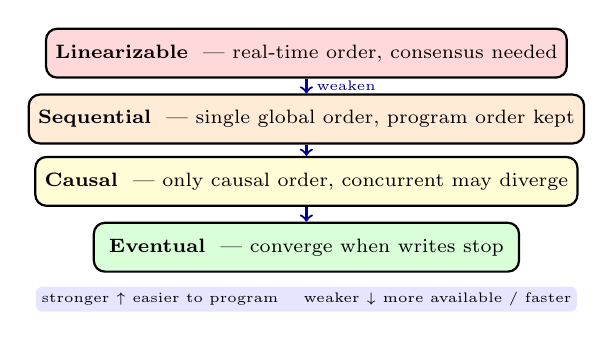
\begin{tikzpicture}[scale=0.88, every node/.style={font=\scriptsize},
  lev/.style={draw,rounded corners=4pt,minimum width=5.4cm,minimum height=0.62cm,align=center,thick}]
\node[lev,fill=red!15] (lin) at (0,2.0) {\textbf{Linearizable} \ --- real-time order, consensus needed};
\node[lev,fill=orange!16] (seq) at (0,1.05) {\textbf{Sequential} \ --- single global order, program order kept};
\node[lev,fill=yellow!16] (cau) at (0,0.15) {\textbf{Causal} \ --- only causal order, concurrent may diverge};
\node[lev,fill=green!15] (eve) at (0,-0.80) {\textbf{Eventual} \ --- converge when writes stop};
\draw[->,thick,blue!60!black] (lin) -- (seq) node[midway,right,font=\tiny] {weaken};
\draw[->,thick,blue!60!black] (seq) -- (cau);
\draw[->,thick,blue!60!black] (cau) -- (eve);
\node[font=\tiny,align=center,fill=blue!10,rounded corners=2pt,inner sep=2pt] at (0,-1.55) {stronger $\uparrow$ easier to program \quad weaker $\downarrow$ more available / faster};
\end{tikzpicture}
\caption{Consistency spectrum. Moving down trades programmability for latency, throughput and partition availability.}
\label{fig:consistency}
\end{figure}

Choosing a level is an application decision. A bank ledger needs linearizable transfer; a social-media like counter can be eventually consistent; a collaborative editor needs causal (so replies follow their parent) but not linearizable.

\begin{lstlisting}[language=Python]
# Simulating causal delivery with vector clocks (buffer until causally ready)
from collections import defaultdict, deque

def causally_ready(msg_vc, delivered_vc, sender):
    # ready iff msg is next from sender and not ahead on any other entry
    if msg_vc[sender] != delivered_vc[sender] + 1:
        return False
    return all(msg_vc[k] <= delivered_vc[k] for k in range(len(msg_vc)) if k != sender)

# Three messages: m1 from P0, m2 from P1 concurrent, m3 from P1 after seeing m1
delivered = [0,0]
buf = deque([([0,1],1), ([1,0],0), ([1,1],1)])  # out-of-order arrival
while buf:
    vc, sender = buf[0]
    if causally_ready(vc, delivered, sender):
        delivered = [max(delivered[i], vc[i]) for i in range(2)]
        print(f"deliver from P{sender} vc={vc} -> delivered={delivered}")
        buf.popleft()
    else:
        buf.rotate(-1)  # try next
        # in real system: wait for missing predecessor
        if all(not causally_ready(vc,s,delivered) for vc,s in buf):
            break
\end{lstlisting}

% ============================================================
\section{Exercises}
\label{sec:ch02-exercises}
\begin{enumerate}[label=E2.\arabic*, leftmargin=*, itemsep=0.6em]
    \item \textbf{NTP bounds.} Two machines sync via NTP with round-trip $20$\,ms and server processing $2$\,ms. Derive the bound on clock offset. If TrueTime reports $\epsilon=5$\,ms, how long must Spanner's commit-wait hold? Why is an interval better than a point timestamp?
    \item \textbf{Lamport trace.} Three processes exchange messages as in Fig.~\ref{fig:lamport}. Compute Lamport timestamps for every event from scratch. Identify a pair $a,b$ with $C(a)<C(b)$ but $a\not\to b$ and explain why.
    \item \textbf{Vector clock application.} Processes $P_1$ and $P_2$ concurrently write key $x$ with vector clocks $[1,0]$ and $[0,1]$. A replica holds both versions. Show the clocks are incomparable. How does Dynamo-style reconciliation expose this to the application? Propose a merge function for a shopping cart.
    \item \textbf{Consistency hierarchy.} Prove sequential consistency does not imply linearizability with a concrete 2-process execution. Then show causal consistency does not imply sequential with a 3-process example where concurrent writes are seen in different orders.
    \item \textbf{Choosing consistency.} For each workload---(a) seat reservation, (b) page-view counter, (c) chat with replies---choose the weakest consistency that preserves correctness. Justify and name a system or protocol that provides it.
\end{enumerate}

% ============================================================
\section*{Chapter Notes}
Lamport, ``Time, clocks, and the ordering of events in a distributed system'' (CACM, 1978) introduces happens-before and logical clocks. Vector clocks: Fidge (1988) and Mattern (1989) independently. Physical time and TrueTime: Corbett et al., ``Spanner'' (OSDI, 2012). Consistency hierarchy: Lamport (1979) for sequential; Herlihy--Wing (1990) for linearizability; causal memory: Ahamad et al.\ (1995). Comprehensive treatment: Kshemkalyani--Singhal, \emph{Distributed Computing} (2nd ed., Ch.~6--7) and van Steen--Tanenbaum (3rd ed., Ch.~6).

% End of Chapter 2
